% Options for packages loaded elsewhere
\PassOptionsToPackage{unicode}{hyperref}
\PassOptionsToPackage{hyphens}{url}
\PassOptionsToPackage{dvipsnames,svgnames,x11names}{xcolor}
%
\documentclass[
  letterpaper,
  DIV=11,
  numbers=noendperiod]{scrartcl}

\usepackage{amsmath,amssymb}
\usepackage{iftex}
\ifPDFTeX
  \usepackage[T1]{fontenc}
  \usepackage[utf8]{inputenc}
  \usepackage{textcomp} % provide euro and other symbols
\else % if luatex or xetex
  \usepackage{unicode-math}
  \defaultfontfeatures{Scale=MatchLowercase}
  \defaultfontfeatures[\rmfamily]{Ligatures=TeX,Scale=1}
\fi
\usepackage{lmodern}
\ifPDFTeX\else  
    % xetex/luatex font selection
\fi
% Use upquote if available, for straight quotes in verbatim environments
\IfFileExists{upquote.sty}{\usepackage{upquote}}{}
\IfFileExists{microtype.sty}{% use microtype if available
  \usepackage[]{microtype}
  \UseMicrotypeSet[protrusion]{basicmath} % disable protrusion for tt fonts
}{}
\makeatletter
\@ifundefined{KOMAClassName}{% if non-KOMA class
  \IfFileExists{parskip.sty}{%
    \usepackage{parskip}
  }{% else
    \setlength{\parindent}{0pt}
    \setlength{\parskip}{6pt plus 2pt minus 1pt}}
}{% if KOMA class
  \KOMAoptions{parskip=half}}
\makeatother
\usepackage{xcolor}
\setlength{\emergencystretch}{3em} % prevent overfull lines
\setcounter{secnumdepth}{5}
% Make \paragraph and \subparagraph free-standing
\makeatletter
\ifx\paragraph\undefined\else
  \let\oldparagraph\paragraph
  \renewcommand{\paragraph}{
    \@ifstar
      \xxxParagraphStar
      \xxxParagraphNoStar
  }
  \newcommand{\xxxParagraphStar}[1]{\oldparagraph*{#1}\mbox{}}
  \newcommand{\xxxParagraphNoStar}[1]{\oldparagraph{#1}\mbox{}}
\fi
\ifx\subparagraph\undefined\else
  \let\oldsubparagraph\subparagraph
  \renewcommand{\subparagraph}{
    \@ifstar
      \xxxSubParagraphStar
      \xxxSubParagraphNoStar
  }
  \newcommand{\xxxSubParagraphStar}[1]{\oldsubparagraph*{#1}\mbox{}}
  \newcommand{\xxxSubParagraphNoStar}[1]{\oldsubparagraph{#1}\mbox{}}
\fi
\makeatother


\providecommand{\tightlist}{%
  \setlength{\itemsep}{0pt}\setlength{\parskip}{0pt}}\usepackage{longtable,booktabs,array}
\usepackage{calc} % for calculating minipage widths
% Correct order of tables after \paragraph or \subparagraph
\usepackage{etoolbox}
\makeatletter
\patchcmd\longtable{\par}{\if@noskipsec\mbox{}\fi\par}{}{}
\makeatother
% Allow footnotes in longtable head/foot
\IfFileExists{footnotehyper.sty}{\usepackage{footnotehyper}}{\usepackage{footnote}}
\makesavenoteenv{longtable}
\usepackage{graphicx}
\makeatletter
\def\maxwidth{\ifdim\Gin@nat@width>\linewidth\linewidth\else\Gin@nat@width\fi}
\def\maxheight{\ifdim\Gin@nat@height>\textheight\textheight\else\Gin@nat@height\fi}
\makeatother
% Scale images if necessary, so that they will not overflow the page
% margins by default, and it is still possible to overwrite the defaults
% using explicit options in \includegraphics[width, height, ...]{}
\setkeys{Gin}{width=\maxwidth,height=\maxheight,keepaspectratio}
% Set default figure placement to htbp
\makeatletter
\def\fps@figure{htbp}
\makeatother

\KOMAoption{captions}{tableheading}
\makeatletter
\@ifpackageloaded{caption}{}{\usepackage{caption}}
\AtBeginDocument{%
\ifdefined\contentsname
  \renewcommand*\contentsname{Table of contents}
\else
  \newcommand\contentsname{Table of contents}
\fi
\ifdefined\listfigurename
  \renewcommand*\listfigurename{List of Figures}
\else
  \newcommand\listfigurename{List of Figures}
\fi
\ifdefined\listtablename
  \renewcommand*\listtablename{List of Tables}
\else
  \newcommand\listtablename{List of Tables}
\fi
\ifdefined\figurename
  \renewcommand*\figurename{Figure}
\else
  \newcommand\figurename{Figure}
\fi
\ifdefined\tablename
  \renewcommand*\tablename{Table}
\else
  \newcommand\tablename{Table}
\fi
}
\@ifpackageloaded{float}{}{\usepackage{float}}
\floatstyle{ruled}
\@ifundefined{c@chapter}{\newfloat{codelisting}{h}{lop}}{\newfloat{codelisting}{h}{lop}[chapter]}
\floatname{codelisting}{Listing}
\newcommand*\listoflistings{\listof{codelisting}{List of Listings}}
\makeatother
\makeatletter
\makeatother
\makeatletter
\@ifpackageloaded{caption}{}{\usepackage{caption}}
\@ifpackageloaded{subcaption}{}{\usepackage{subcaption}}
\makeatother

\ifLuaTeX
  \usepackage{selnolig}  % disable illegal ligatures
\fi
\usepackage{bookmark}

\IfFileExists{xurl.sty}{\usepackage{xurl}}{} % add URL line breaks if available
\urlstyle{same} % disable monospaced font for URLs
\hypersetup{
  pdftitle={Assignment3},
  pdfkeywords={Quarto, Election Campaigns, Voter Behavior},
  colorlinks=true,
  linkcolor={blue},
  filecolor={Maroon},
  citecolor={Blue},
  urlcolor={Blue},
  pdfcreator={LaTeX via pandoc}}


\title{Assignment3}
\author{Jiacheng Li}
\date{2024-04-09}

\begin{document}
\maketitle
\begin{abstract}
This report analyzes the voter information for the top three candidates
in terms of donations and voter support of Barack Obama, Ron Paul, and
Mitt Romney.
\end{abstract}


\section{Introduction}\label{introduction}

In modern election campaigns, data analysis plays a crucial role in
understanding voter behavior and financial contributions. By examining
voting patterns and donation distributions, we can gain insights into
the support base of leading candidates. This report focuses on analyzing
the voter information for the top three candidates based on the number
of votes received: Barack Obama, Ron Paul, and Mitt Romney. The analysis
primarily focuses on the distribution of voters and their spending
patterns.

\section{Top 3 Candidates}\label{top-3-candidates}

\subsection{Summary}\label{summary}

In terms of both donation amount and donor count, Obama, Romney, and
Paul rank among the top three candidates. Therefore, we focus our
analysis on the voter information of these three candidates.

\subsection{Donors}\label{donors}

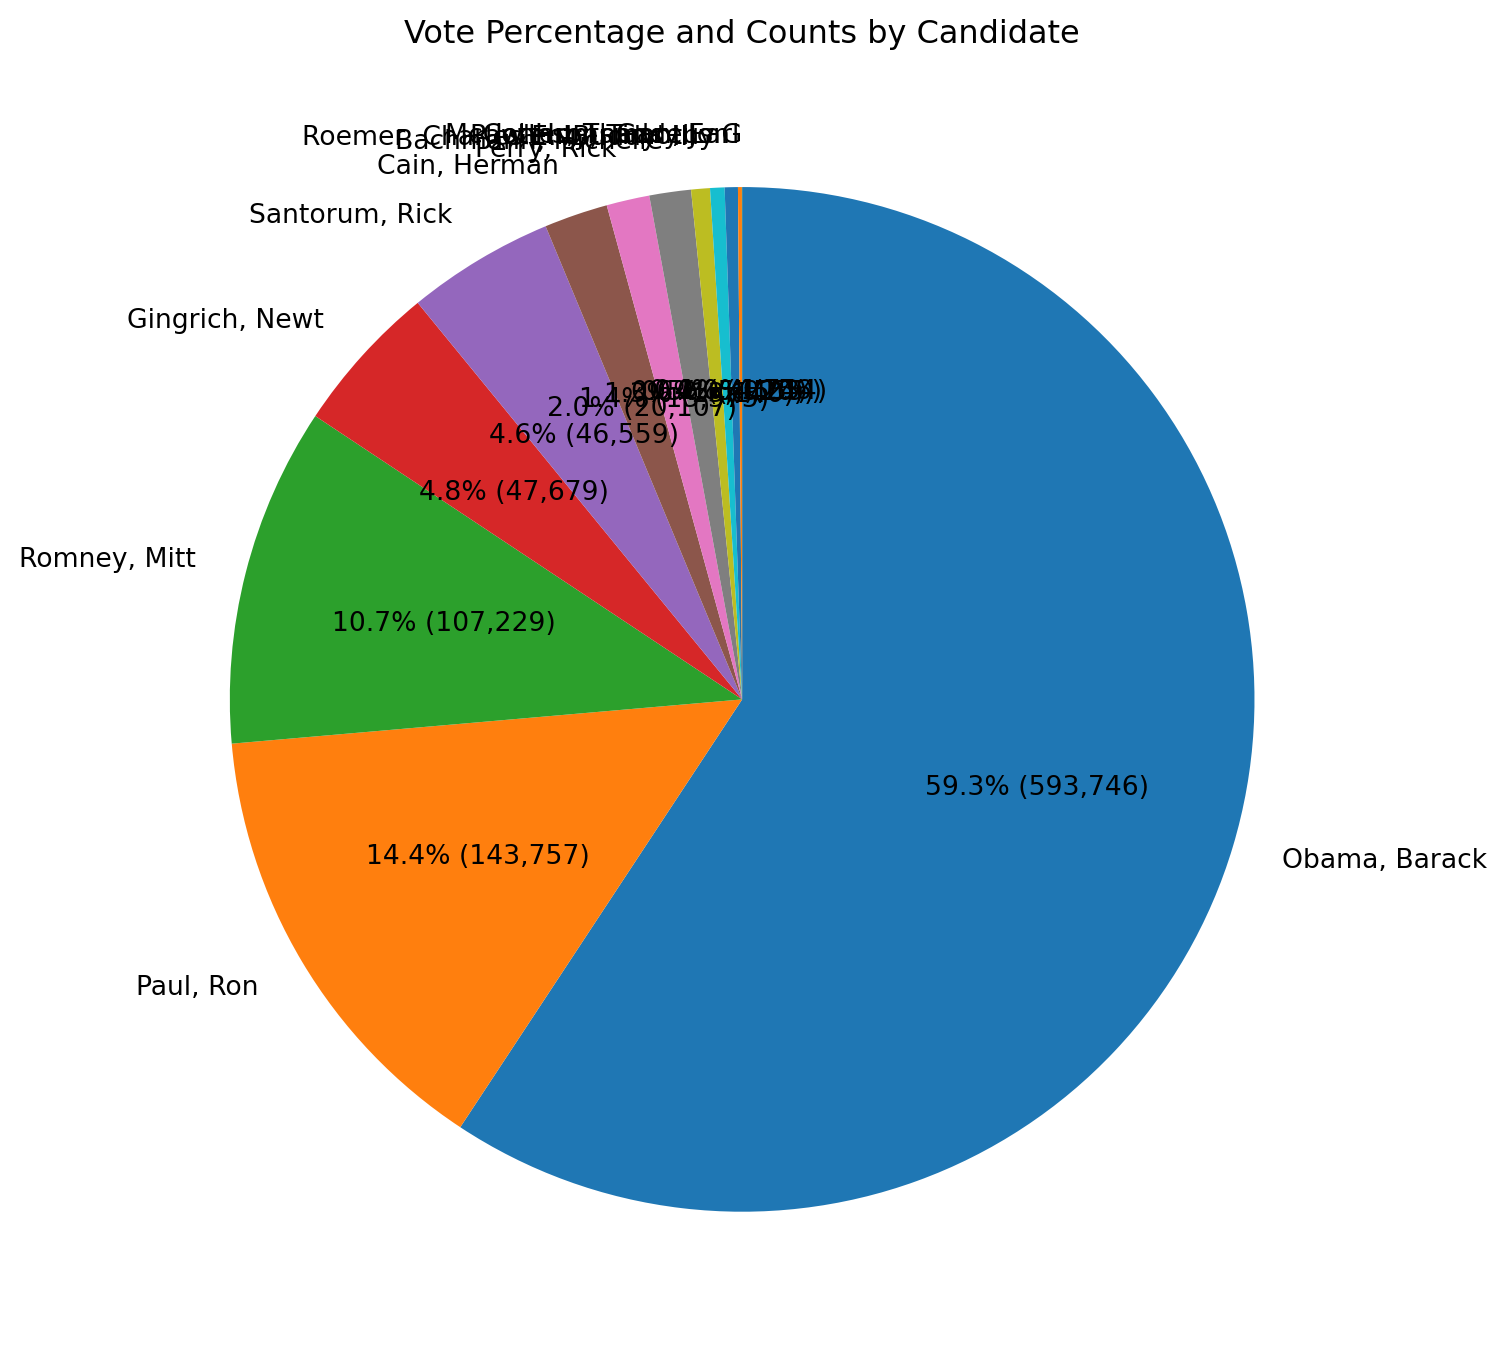
\includegraphics{0_main_file_files/figure-pdf/cell-2-output-2.pdf}

\subsection{Contributions}\label{contributions}

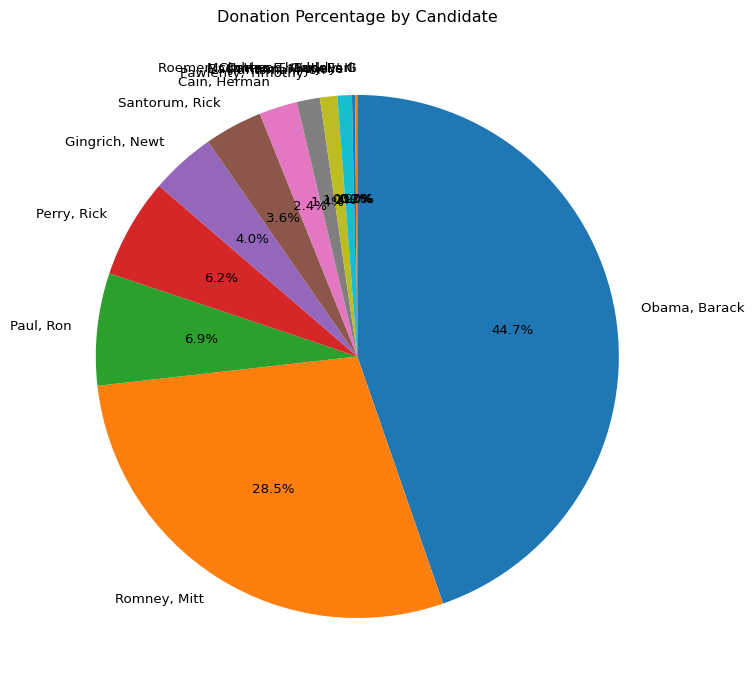
\includegraphics{0_main_file_files/figure-pdf/cell-3-output-1.pdf}

\section{Statewise Total Donations for Barack Obama, Ron Paul, and Mitt
Romney}\label{statewise-total-donations-for-barack-obama-ron-paul-and-mitt-romney}

\subsection{Summary}\label{summary-1}

Overall, Obama leads in donations across both large and small states,
reflecting his broader nationwide support. Romney, on the other hand,
relies on donations from a few key states, indicating a more
concentrated and elite-based fundraising structure. Paul's grassroots
supporters, though widespread, contribute smaller amounts overall.

\subsection{Barack Obama}\label{barack-obama}

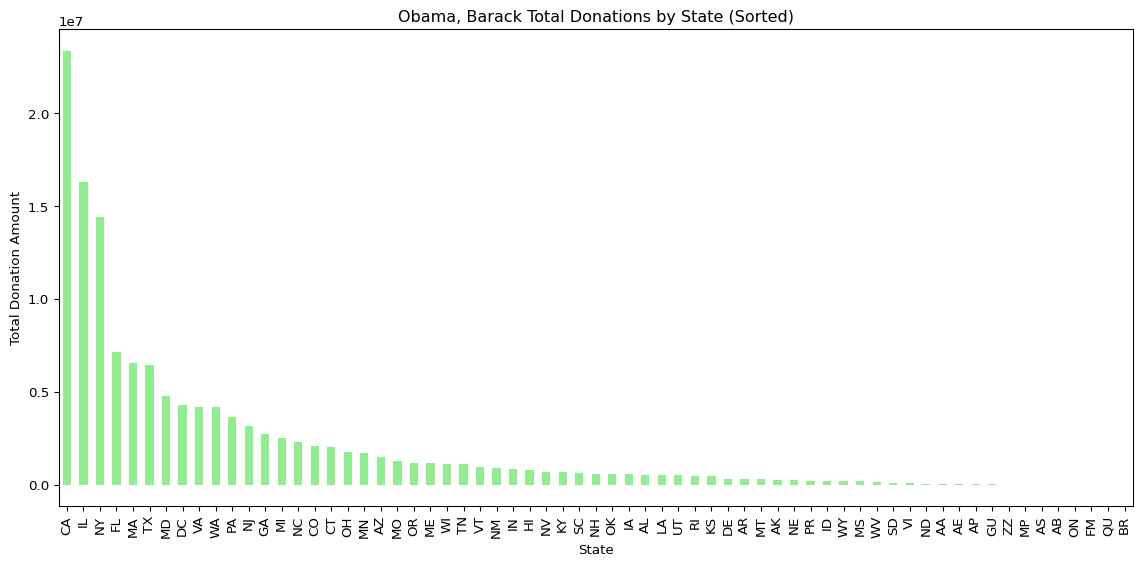
\includegraphics{0_main_file_files/figure-pdf/cell-4-output-1.pdf}

\subsection{Ron Paul}\label{ron-paul}

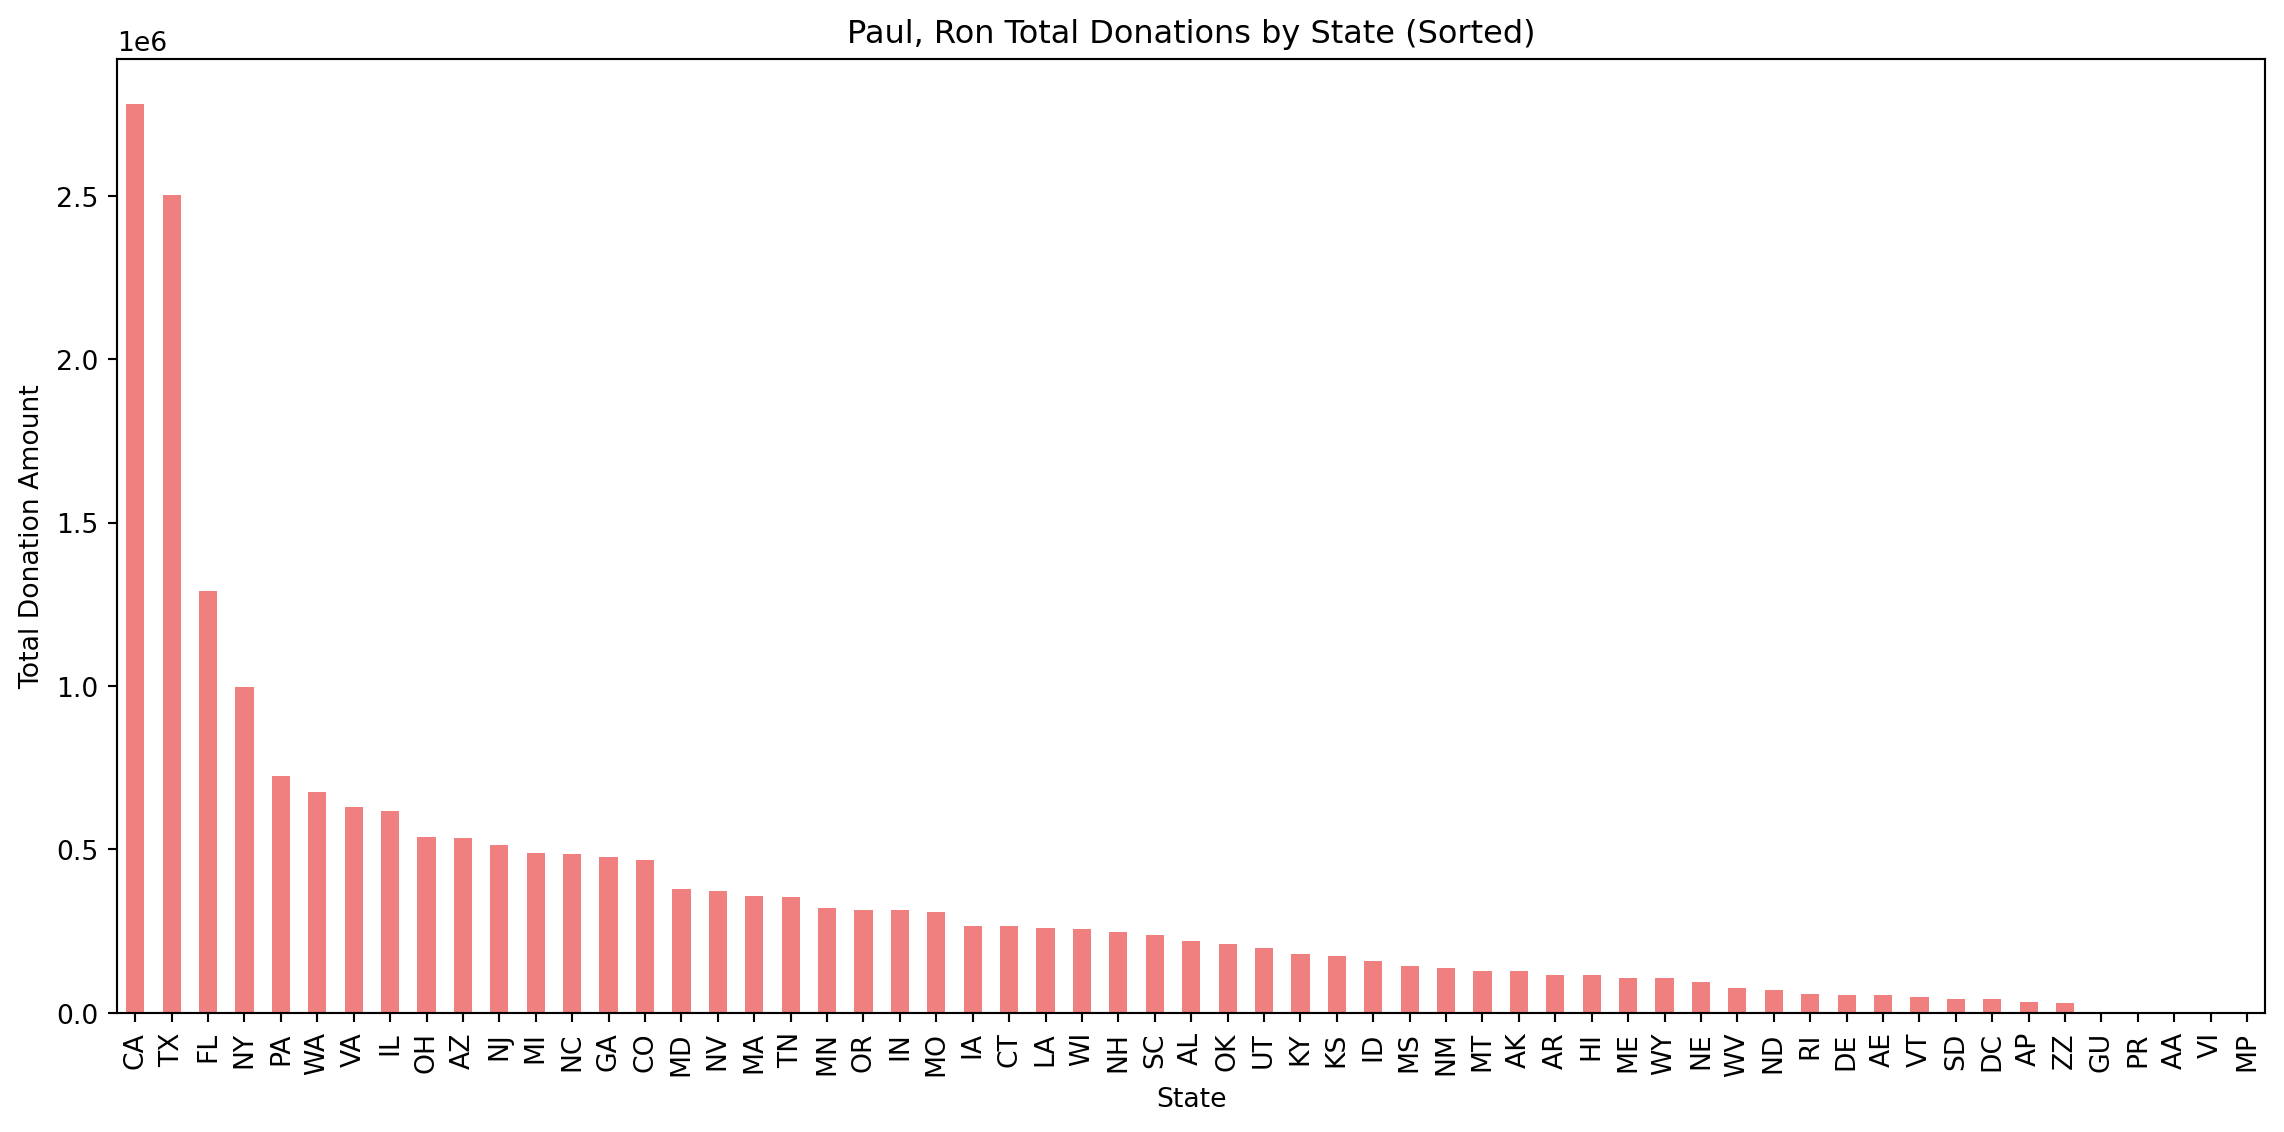
\includegraphics{0_main_file_files/figure-pdf/cell-5-output-1.pdf}

\subsection{Mitt Romney}\label{mitt-romney}

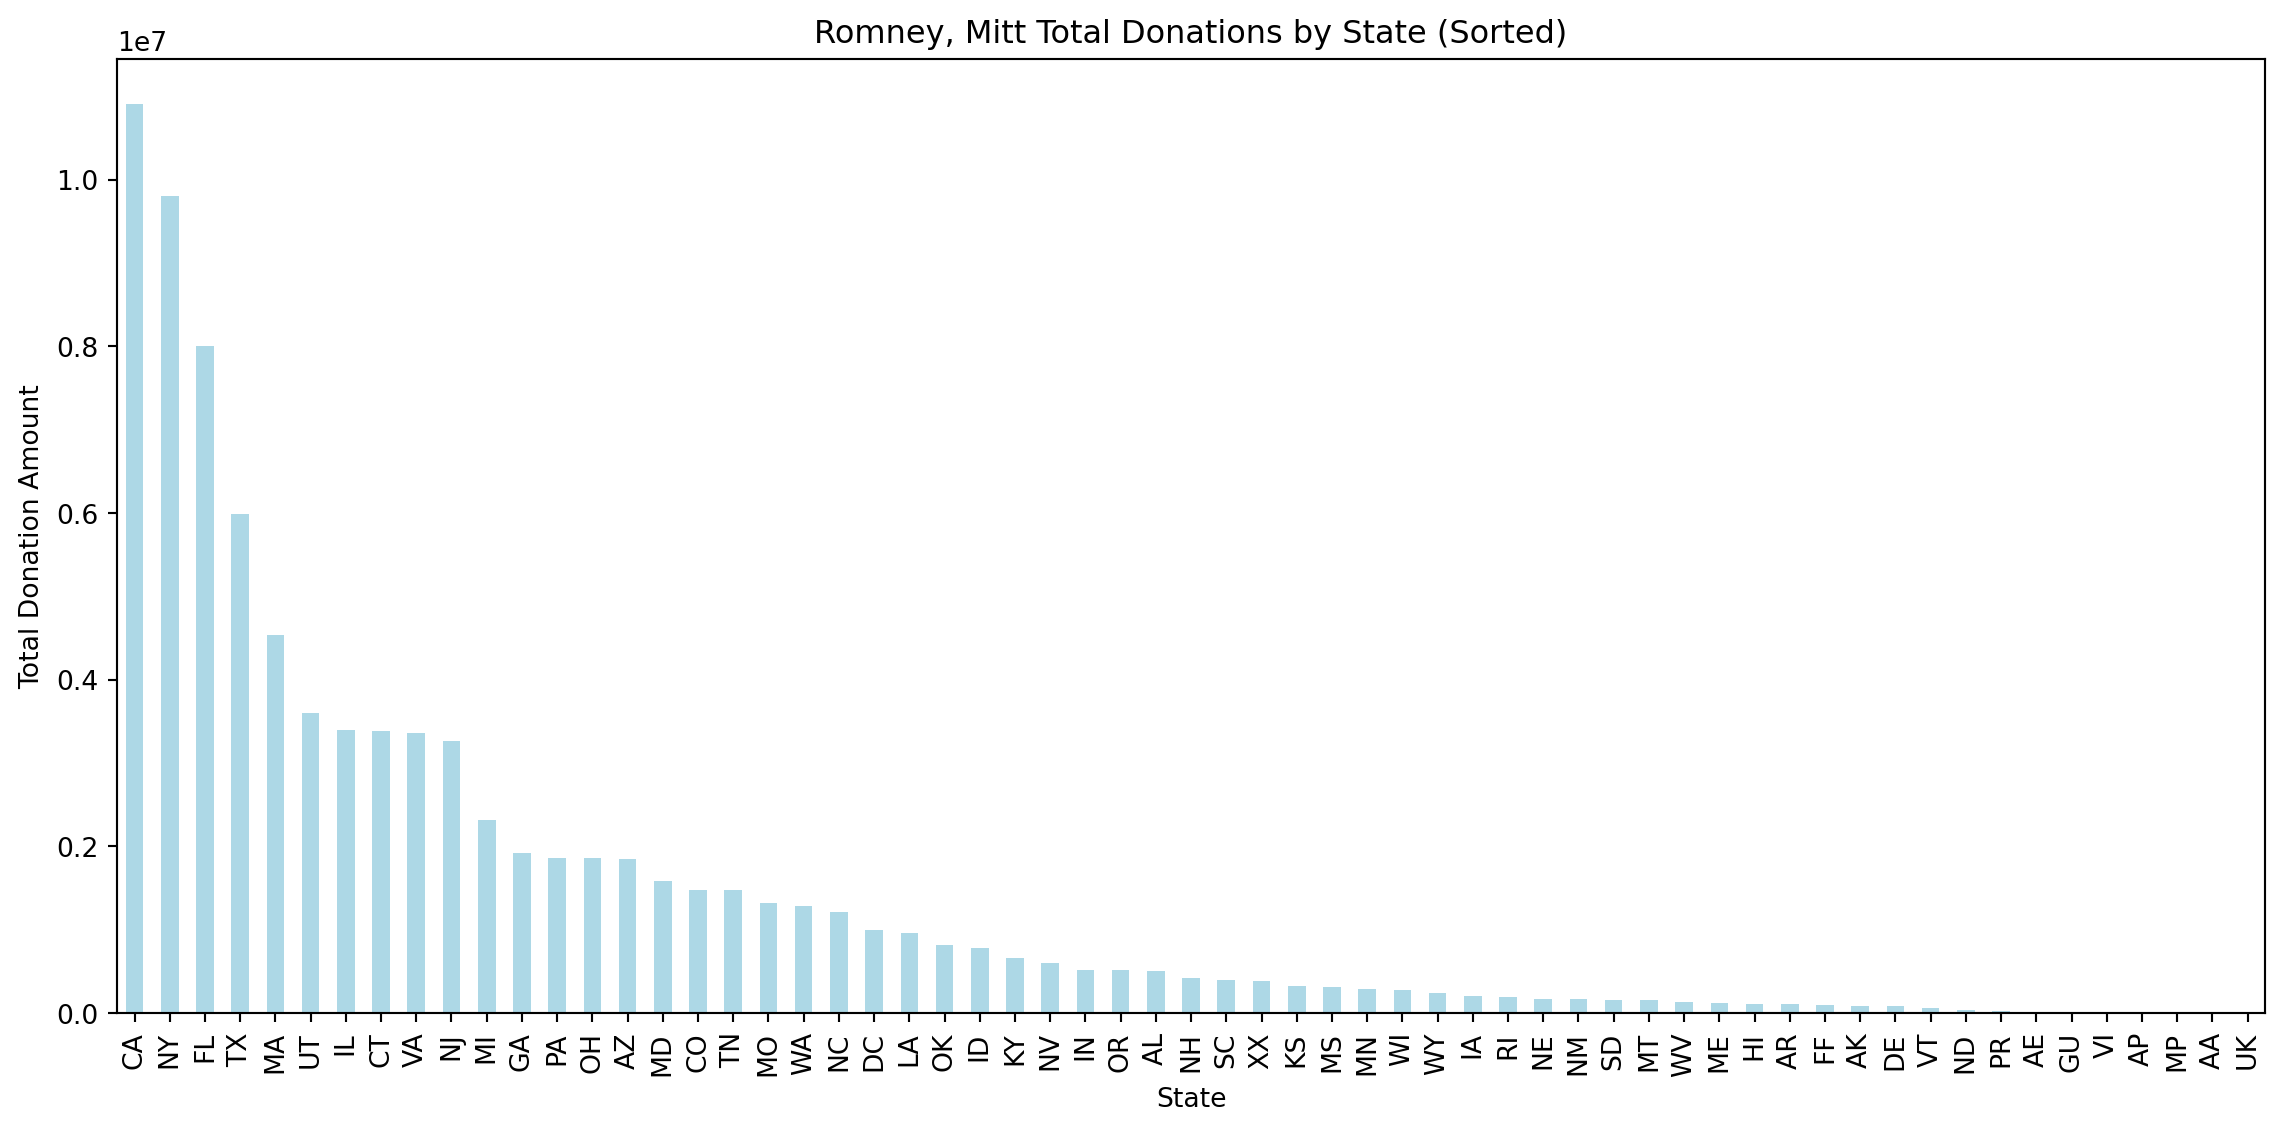
\includegraphics{0_main_file_files/figure-pdf/cell-6-output-1.pdf}

\section{Average Donation Amount per State for Barack Obama, Ron Paul,
and Mitt
Romney}\label{average-donation-amount-per-state-for-barack-obama-ron-paul-and-mitt-romney}

\subsection{Summary}\label{summary-2}

Romney heavily relies on large donations from a few contributors,
particularly excelling in certain key states. This fundraising strategy
seems to depend on a more elite network of donors. On the other hand,
Obama draws more from small donations by ordinary voters. Although his
average donation is lower than Romney's, his broad nationwide support
gives him a strong competitive advantage in fundraising. Paul's donor
base is widespread but with limited funding, indicating that his
supporters primarily contribute smaller amounts, which puts him at a
disadvantage in overall fundraising efforts.

\subsection{Barack Obama}\label{barack-obama-1}

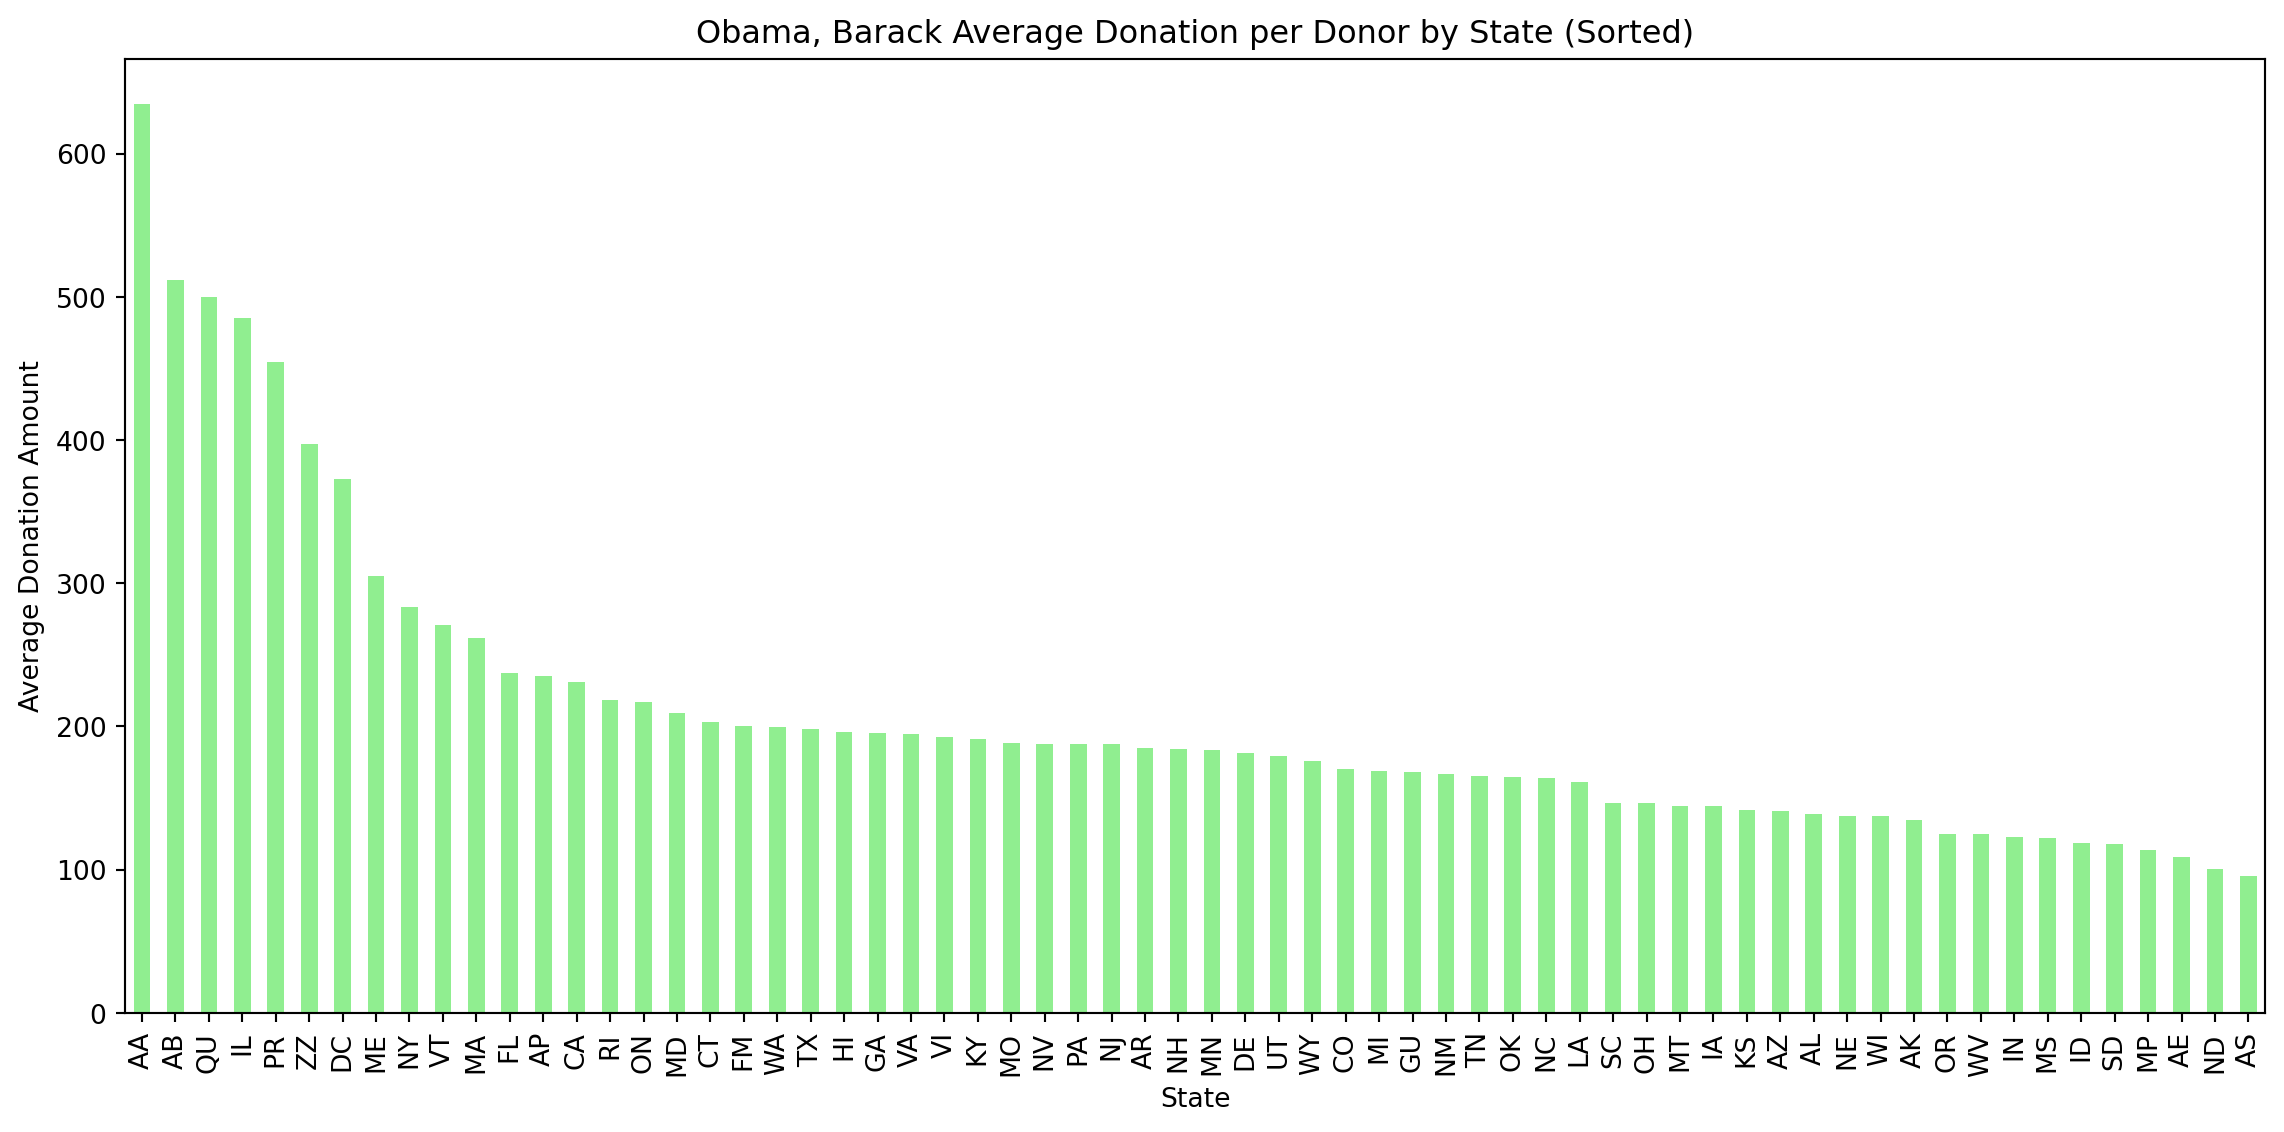
\includegraphics{0_main_file_files/figure-pdf/cell-7-output-1.pdf}

\subsection{Ron Paul}\label{ron-paul-1}

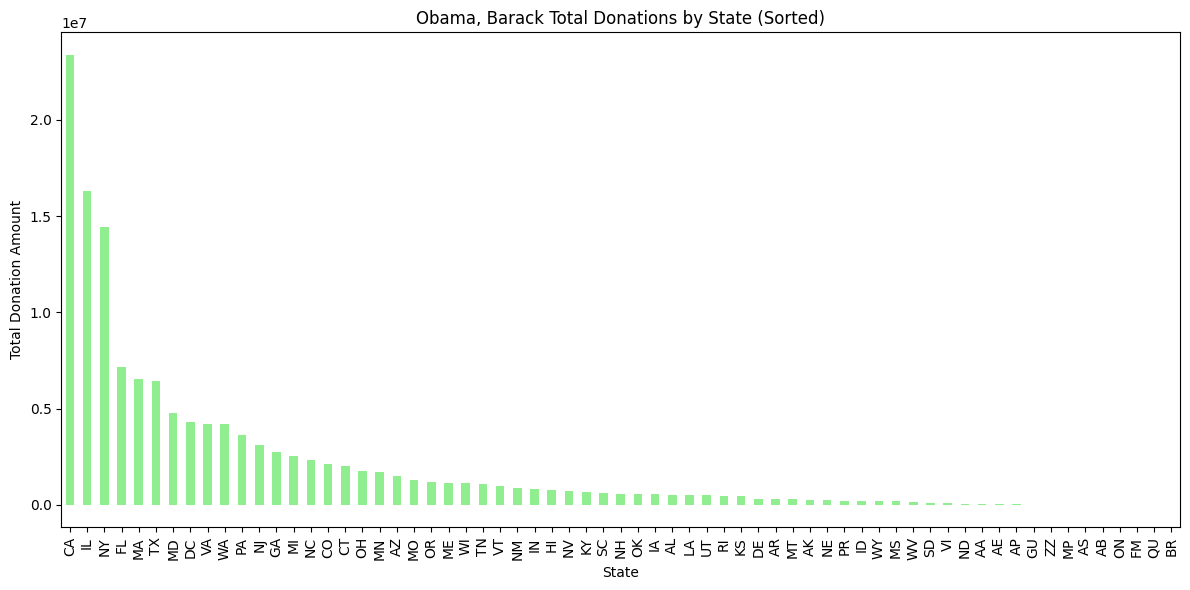
\includegraphics{0_main_file_files/figure-pdf/cell-8-output-1.pdf}

\subsection{Mitt Romney}\label{mitt-romney-1}

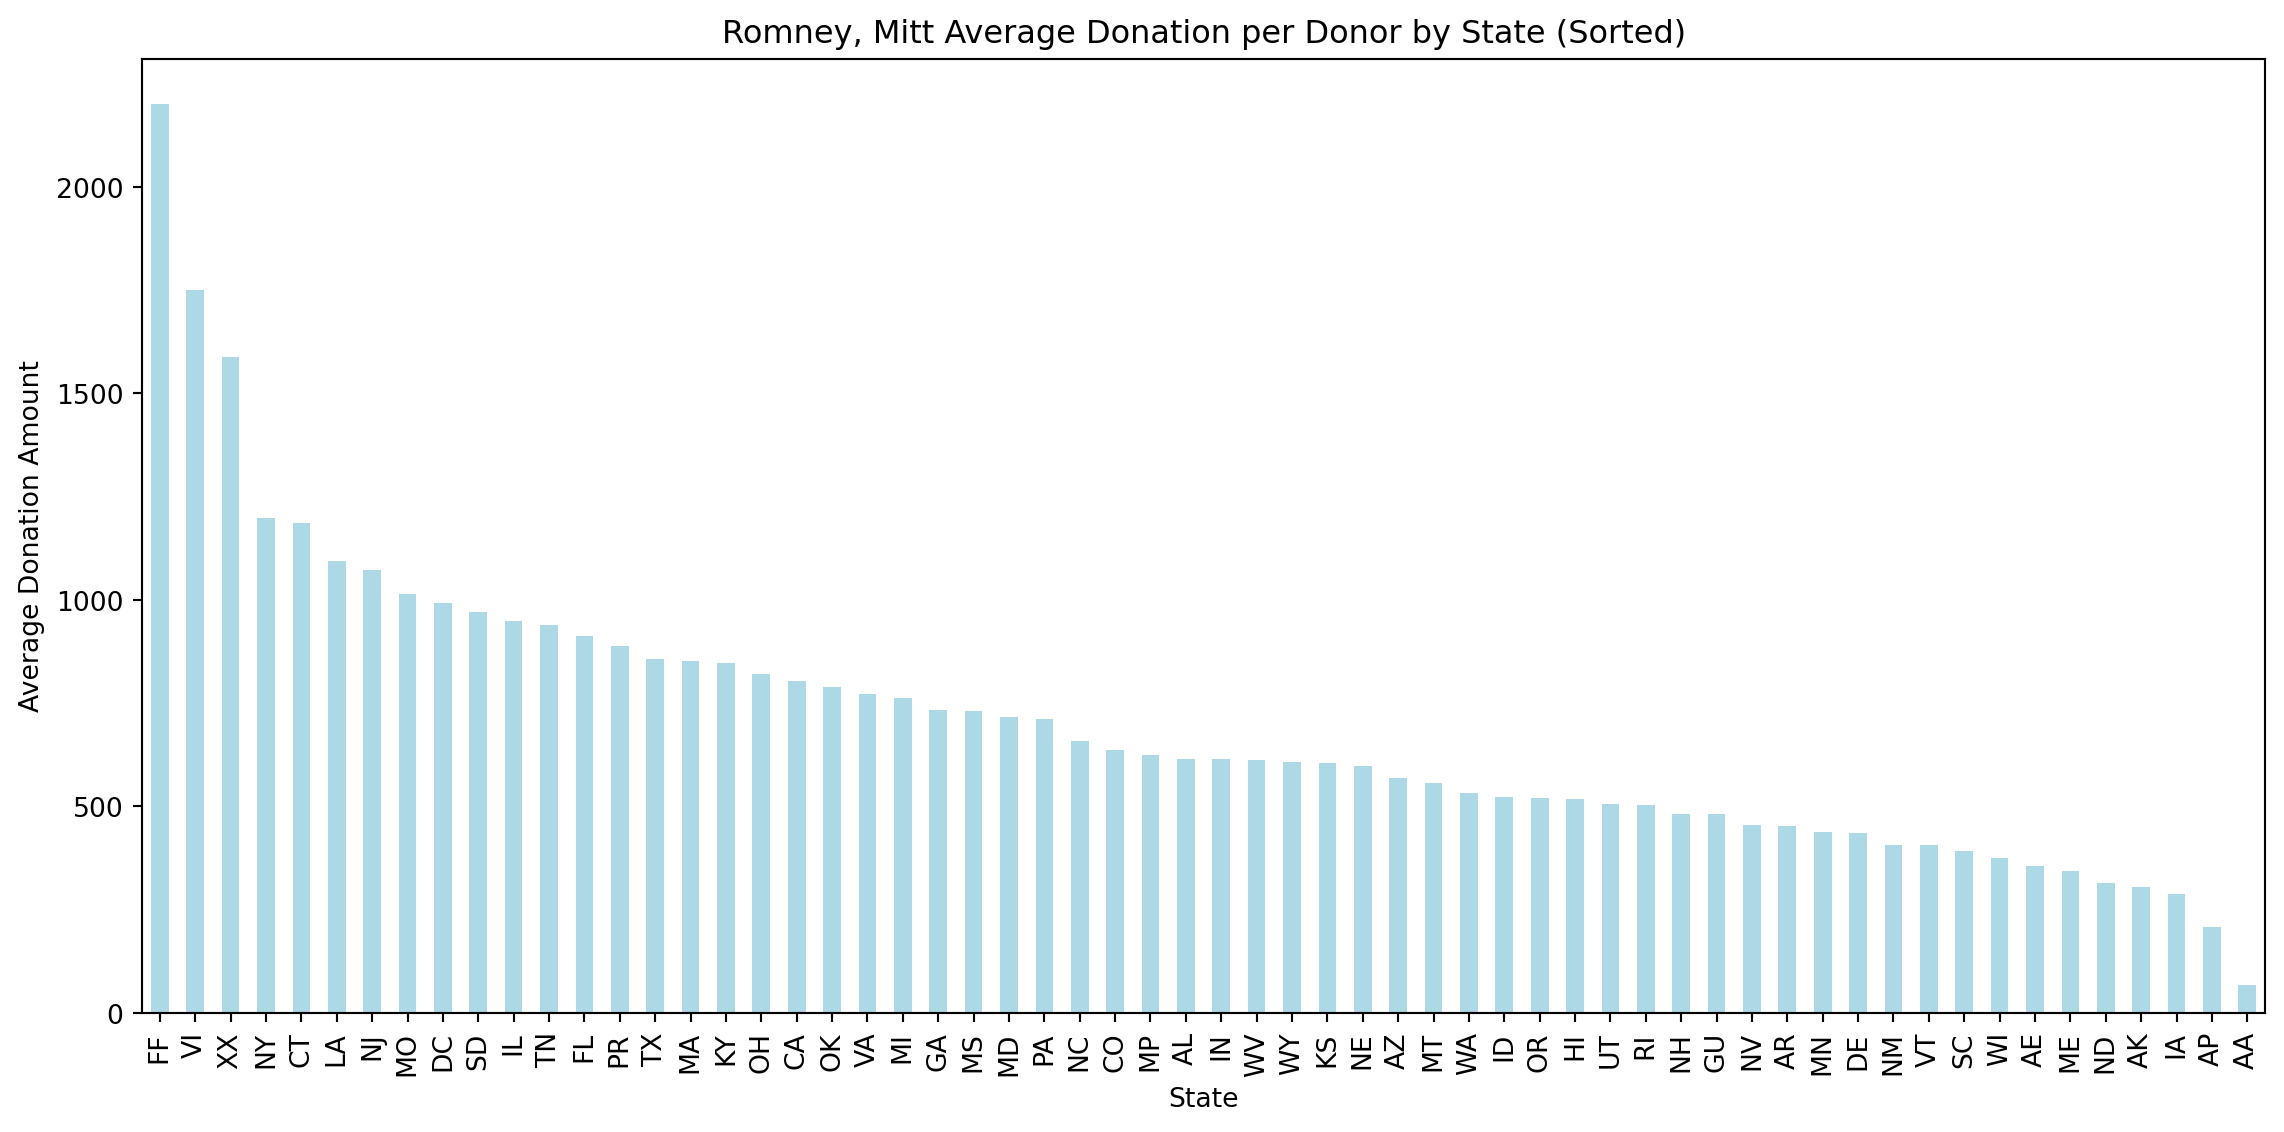
\includegraphics{0_main_file_files/figure-pdf/cell-9-output-1.pdf}

\subsection{Overall}\label{overall}

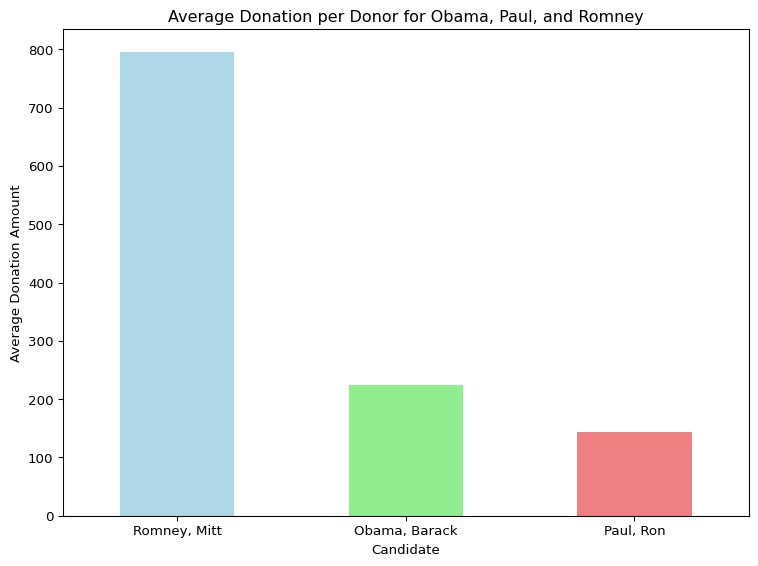
\includegraphics{0_main_file_files/figure-pdf/cell-10-output-1.pdf}

\section{Vote Share by State for Barack Obama, Ron Paul, and Mitt
Romney}\label{vote-share-by-state-for-barack-obama-ron-paul-and-mitt-romney}

\subsection{Summary}\label{summary-3}

Obama has a broader support base in most states, with the largest
percentage of donors. Romney's support is concentrated in a few key
states, where he demonstrates a strong regional advantage. Paul's
supporters are more widely distributed, but their proportion is
relatively low, indicating that while he has widespread grassroots
support, his overall influence is not as strong as Obama's or Romney's.

\subsection{Overall}\label{overall-1}

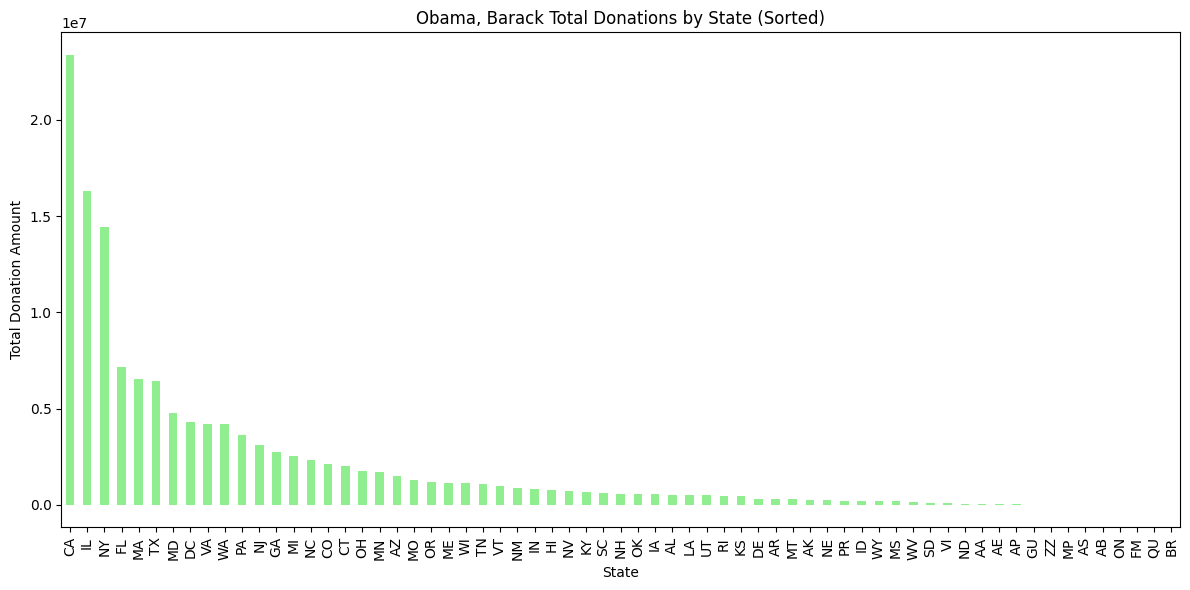
\includegraphics{0_main_file_files/figure-pdf/cell-11-output-1.pdf}

\section{Conclusion}\label{conclusion}

In this report, we analyzed the voter information for the top three
candidates, Barack Obama, Ron Paul, and Mitt Romney, focusing on their
statewise donations, average donation amounts, and vote shares. The data
reveals clear differences in the support bases and fundraising
strategies of each candidate.

Obama's broad national appeal is evident from his widespread support
across both large and small states, where he consistently led in both
donor numbers and total contributions. His reliance on smaller
individual donations underscores his broad, grassroots appeal, providing
him with a competitive advantage across the country.

Romney's fundraising efforts, while also significant, are more
concentrated in key states, suggesting a reliance on high-net-worth
donors. His ability to attract large donations in a few critical areas
highlights his regional strengths, but this strategy may limit his
broader appeal compared to Obama.

Paul, though widely supported by grassroots donors, faces challenges in
fundraising due to the relatively smaller contribution amounts. While
his support is spread across many states, the overall financial backing
he receives is less robust than that of his competitors, which may
impact his ability to maintain competitiveness.

In summary, the distribution of voter support and donation patterns
clearly differentiates these three candidates, with Obama showing the
broadest and most balanced support, Romney excelling in high-value
contributions from key states, and Paul drawing more modest
contributions from a wide, grassroots base.




\end{document}
